\documentclass[11pt]{article}

%% MinionPro fonts 
%\usepackage[lf]{MinionPro}
%\usepackage{MnSymbol}
\usepackage{microtype}

%% Margins
\usepackage{geometry}
\geometry{verbose,letterpaper,tmargin=1in,bmargin=1in,lmargin=1in,rmargin=1in}

%% Other packages
\usepackage{amsmath}
\usepackage{amsthm}
\usepackage[shortlabels]{enumitem}
\usepackage{titlesec}
\usepackage{soul}
\usepackage{tikz}
\usepackage{mathtools}
\usepackage{pgfplots}
\usepackage{tikz-3dplot}
\usepackage{algorithmic}
\usepackage[export]{adjustbox}
\usepackage{tcolorbox}
\usepackage{mathrsfs}

%% Paragraph style settings
\setlength{\parskip}{\medskipamount}
\setlength{\parindent}{0pt}

%% Change itemize bullets
\renewcommand{\labelitemi}{$\bullet$}
\renewcommand{\labelitemii}{$\circ$}
\renewcommand{\labelitemiii}{$\diamond$}
\renewcommand{\labelitemiv}{$\cdot$}

%% Colors
\definecolor{rred}{RGB}{204,0,0}
\definecolor{ggreen}{RGB}{0,145,0}
\definecolor{yyellow}{RGB}{255,185,0}
\definecolor{bblue}{rgb}{0.2,0.2,0.7}
\definecolor{ggray}{RGB}{190,190,190}
\definecolor{ppurple}{RGB}{160,32,240}
\definecolor{oorange}{RGB}{255,165,0}

%% Shrink section fonts
\titleformat*{\section}{\normalsize\bf}
\titleformat*{\subsection}{\normalsize\bf}
\titleformat*{\subsubsection}{\normalsize\it}

% %% Compress the spacing around section titles
\titlespacing*{\section}{0pt}{1.5ex}{0.75ex}
\titlespacing*{\subsection}{0pt}{1ex}{0.5ex}
\titlespacing*{\subsubsection}{0pt}{1ex}{0.5ex}

%% amsthm settings
\theoremstyle{definition}
\newtheorem{problem}{Problem}
\newtheorem{example}{Example}
\newtheorem*{theorem}{Theorem}
\newtheorem*{bigthm}{Big Theorem}
\newtheorem*{biggerthm}{Bigger Theorem}
\newtheorem*{bigcor1}{Big Corollary 1}
\newtheorem*{bigcor2}{Big Corollary 2}

%% tikz settings
\usetikzlibrary{calc}
\usetikzlibrary{patterns}
\usetikzlibrary{decorations}
\usepgfplotslibrary{polar}

%% algorithmic setup
\algsetup{linenodelimiter=}
\renewcommand{\algorithmiccomment}[1]{\quad// #1}
\renewcommand{\algorithmicrequire}{\emph{Input:}}
\renewcommand{\algorithmicensure}{\emph{Output:}}

%% Answer box macros
%% \answerbox{alignment}{width}{height}
\newcommand{\answerbox}[3]{%
  \fbox{%
    \begin{minipage}[#1]{#2}
      \hfill\vspace{#3}
    \end{minipage}
  }
}

%% \answerboxfull{alignment}{height}
\newcommand{\answerboxfull}[2]{%
  \answerbox{#1}{6.38in}{#2} 
}

%% \answerboxone{alignment}{height} -- for first-level bullet
\newcommand{\answerboxone}[2]{%
  \answerbox{#1}{6.0in}{#2} 
}

%% \answerboxtwo{alignment}{height} -- for second-level bullet
\newcommand{\answerboxtwo}[2]{%
  \answerbox{#1}{5.8in}{#2}
}

%% special boxes
\newcommand{\wordbox}{\answerbox{c}{1.2in}{.7cm}}
\newcommand{\catbox}{\answerbox{c}{.5in}{.7cm}}
\newcommand{\letterbox}{\answerbox{c}{.7cm}{.7cm}}

%% Miscellaneous macros
\newcommand{\tstack}[1]{\begin{multlined}[t] #1 \end{multlined}}
\newcommand{\cstack}[1]{\begin{multlined}[c] #1 \end{multlined}}
\newcommand{\ccite}[1]{\only<presentation>{{\scriptsize\color{gray} #1}}\only<article>{{\small [#1]}}}
\newcommand{\grad}{\nabla}
\newcommand{\ra}{\ensuremath{\rightarrow}~}
\newcommand{\maximize}{\text{maximize}}
\newcommand{\minimize}{\text{minimize}}
\newcommand{\subjectto}{\text{subject to}}
\newcommand{\trans}{\mathsf{T}}
\newcommand{\bb}{\mathbf{b}}
\newcommand{\bx}{\mathbf{x}}
\newcommand{\bc}{\mathbf{c}}
\newcommand{\bd}{\mathbf{d}}

%% LP format
%    \begin{align*}
%      \maximize \quad & \mathbf{c}^{\trans} \mathbf{x}\\
%      \subjectto \quad & A \mathbf{x} = \mathbf{b}\\
%                       & \mathbf{x} \ge \mathbf{0}
%    \end{align*}


%% Redefine maketitle
\makeatletter
\renewcommand{\maketitle}{
  \noindent SA405 -- AMP \hfill Rader \S 4.1 \\

  \begin{center}\Large{\textbf{\@title}}\end{center}
}
\makeatother

%% ----- Begin document ----- %%
\begin{document}
  
\title{Lesson 12.  Vehicle Routing Problem (VRP)}

\maketitle

%%%
\section{Today...}

\begin{itemize}
	\item  Description of the Vehicle Routing Problem
	\item  Pizza Delivery Example
\end{itemize}

\section{VRP:  An extension of TSP}

\textbf{Vehicle Routing Problems} are similar to TSP, except that instead of having a single ``salesperson'', we have multiple ``salespeople'', all \emph{starting and ending at the same location}.  We must decide the ``cheapest'' way to cover all of the locations via tours with our fleet of salespeople.

\begin{problem} The pizza restaurant at {\huge ${\star}$} has 12 delivery orders ready and three drivers.  Each driver can serve at most 5 customers.  Draw a \emph{feasible} solution to the VRP problem on the graph below.

\vspace{.5cm}
\begin{center}
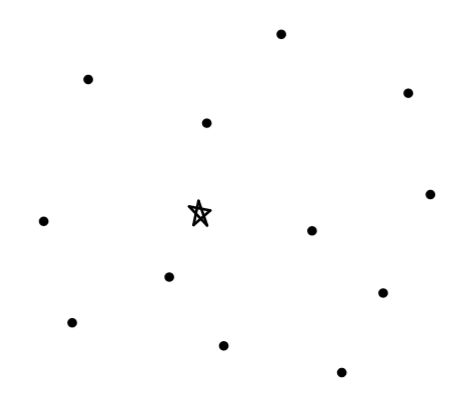
\includegraphics[width=0.7\textwidth]{big_graph}
\end{center}
\end{problem}

%\bigskip
%\begin{tcolorbox}
%Vehicle routing is a very practical real world application.
%\end{tcolorbox}

\begin{problem} Think of a real world vehicle routing application.  Can you think of a the name of a company that faces this problem?\\
\answerboxfull{c}{,5in}
\end{problem}

\newpage

The following are the assumptions of a basic Vehicle Routing Problem:

\begin{itemize}
	\item We have a fixed number of vehicles.
	\item All vehicles start and end a common location, or \textbf{depot}.
	\item All vehicles have the same capacity.  
	\item Vehicles may serve many different customers, up to capacity.
	\item Each customer's demand must be served by a single vehicle.
	\item Goal:  Find a minimum cost collection of \emph{tours}, all starting and ending at the depot, that contain all customers and do not violate vehicle capacities.
\end{itemize}




\begin{tcolorbox}
\textbf{Basic VRP:  Mathematical Description}

Notation: 
\begin{itemize}
	\item Let $G = (V,E)$ be an undirected graph.  
		\begin{itemize}
			\item One of the vertices is distinguished as the \emph{depot}: usually vertex ``$0$''.
			\item Each edge has a cost (or distance): $c_{ij} \ge 0,$ for $(i,j) \in E$.
			\item Each vertex has a demand: $d_i >0$, for $i \in V$.
		\end{itemize}
	\item  Exactly $m$ tours (vehicles) used, each with the same demand capacity ($D >0$).
\end{itemize}

Requirements:
\begin{itemize}
	\item Each tour must include the depot.
	\item Each vertex (customer) must be be served.
	\item The total demand of all the customers served on each tour must not exceed $D$.
\end{itemize}

Formulation assumptions:
\begin{itemize}
	\item Every vehicle visits at least two customers.
	\item The direction an edge is traversed does not affect the cost.
	\item (Variations of the formulation can work around these assumptions.)
\end{itemize}
Goal:
\begin{itemize}
	\item  Minimize total cost of tours.
\end{itemize}
\end{tcolorbox}


VRP can be modified to incorporate variations including:
\begin{itemize}
\item \textbf{VRP with time windows:}  Each customer must be visited within a certain time window.
\item \textbf{Multidepot VRP:}  Fixed number of vehicles starting at each of multiple depots. 
\item \textbf{Split deliver VRP: } Customer demand can be met by more than one vehicle
\end{itemize}

\newpage

\section{Pizza Deliveries (Example 4.1 in Rader)}

A local pizza shop received 10 late orders for delivery last night; unfortunately,
only three delivery persons are working.  The pizza shop is labeled node 0.  The 10 delivery locations are labeled $\{1,2,3,\dots,10\}$.  Suppose the distance between location $i$ and location $j$ is $c_{ij}$ (no matter which direction the route is traveled).  Assuming that each driver can deliver at most four orders, how should the delivery
routes be determined in order to minimize the total travel distance?

\begin{problem}
Write a concrete formulation for the pizza delivery VRP that includes only the constraints that specify the required degree at each node.  \textbf{This formulation is incomplete.}  \emph{Use the usual  naming convention for edges:  there is an edge $(i,j)$ for every pair of locations $i$ and $j$ such that $i < j$.}

\answerboxfull{c}{8cm}
\end{problem}



\begin{problem}
Suppose a solution to the incomplete model above contains cycles on the vertices $\{0,2,4\}, \{0,6,9\}, \{0,8,10\},$ and $\{1,3,5,7\}$. 
\begin{enumerate}[(a)]
\item Why is the solution infeasible to the (complete) VRP formulation?  \\
\answerboxone{c}{0.4in}
\item Write a concrete constraint that would eliminate this solution from the feasible region.\\
\answerboxone{c}{1in}
\end{enumerate}
\end{problem}

\newpage
\begin{problem}
Suppose a solution to the incomplete model above contains cycles on the vertices $\{0,2,4\}, \{0,6,9\},$ and $\{0,1,3,5,7,8,10\}$. 
\begin{enumerate}[(a)]
\item Why is the solution infeasible to the (complete) VRP formulation?  \\
\answerboxone{c}{0.4in}
\item Write a concrete constraint that would eliminate this solution from the feasible region.\\
\answerboxone{c}{1in}
\end{enumerate}
\end{problem}

\begin{problem}
Write a \textbf{complete} abstract formulation for the pizza delivery VRP that includes the \emph{generalized subtour elimination constriants}.  Use the ``Route splitting'' section on the last page of the notes to discover the correct right-hand side for the generalized subtour elimination constraints.\\
\answerboxfull{c}{10cm}
\end{problem}

\section{Solving VRP Iteratively}  
\begin{problem}Which set of constraints must be added iteratively and why?

\answerboxfull{c}{2cm}
\end{problem}

\section{Route splitting}

How many edges must we include among $|S|$ vertices in order to have $C$ connected components and NO CYCLES?  (This assumes that $C$ vehicles are required to visit the set of locations, due to vehicle capacity.)  Let's try some test cases...

\begin{description}
\item{$C = 1$:}  How many edges must we include in order to have 1 connected component and no cycles?

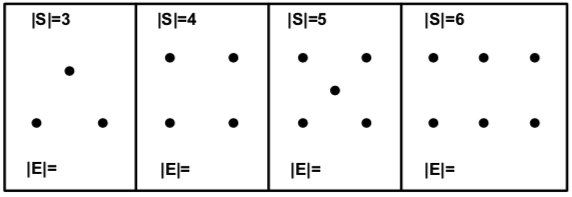
\includegraphics[width = 0.8\textwidth]{four_graphs.png}

\vfill
\item{$C = 2$:}  How many edges must we include in order to have 2 connected component and no cycles?

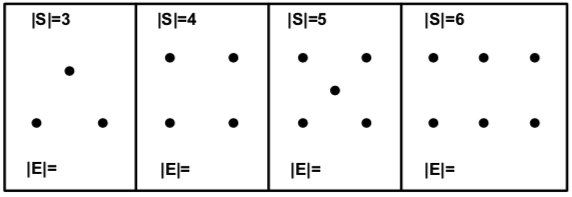
\includegraphics[width = 0.8\textwidth]{four_graphs.png}

\vfill

\item{$C = 3$:}  How many edges must we include in order to have 3 connected component and no cycles?

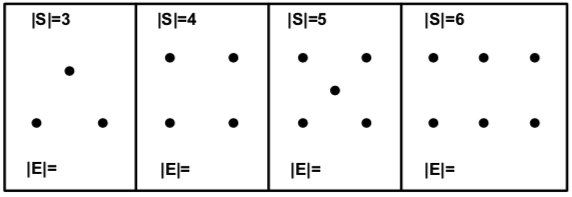
\includegraphics[width = 0.8\textwidth]{four_graphs.png}

\vfill
\item{General $C> 0$:} How many edges must we include among $|S|$ vertices in order to have $C$ connected components and NO CYCLES?

\answerboxfull{c}{2cm}

\vfill
\end{description}



\end{document}



